\chapter{Zielarchitektur}
\label{ch:TARGET}

Im Rahmen dieses Kapitels wird der unter anderem aus dieser Arbeit resultierende Stand der Architektur von \textit{Zeta} beschrieben. Um genau zu sein wird der Stand aus dem Commit 00098eaab05231f23bf35d1dab79a240e55d1efc vom 17.03.2018 beschrieben \cite{zeta_new}. Dabei wird im speziellen auf die Änderung bzw. Erweiterungen an der Architektur im Vergleich zur Ausgangsarchitektur eingegangen. Zu Beginn wird auf das Frontend mit seinen Teilanwendungen wie den Code-Editor, den Concept-Editor, Model-Editor und der Webapp eingegangen. Anschließend wird das Backend mit seiner Laufzeitumgebung, der Qualitätssicherung, einigen Teilkomponenten des \textit{Play Servers} und der Generator Verwaltung mit der Ausführung der Generatoren beschrieben.

\section{Front-End}

Das Frontend besteht weiterhin, wie zuvor im Abschnitt~\ref{sec:INITIAL_FRONTEND} ab Seite~\pageref{sec:INITIAL_FRONTEND} beschrieben, zum einen aus primär statischen Seiten zur Anmeldung oder der Verwaltung der Projekte. Zum anderen aus einer Reihe von browserseitigen Anwendungen wie dem Code-Editor, den Graphischen Editoren und der Webapp. Die Abbildung~\ref{fig:ZETA_OVERVIEW_NEW} auf Seite~\pageref{fig:ZETA_OVERVIEW_NEW} ist eine Übersicht dieser Anwendung aus dem Frontend mit den Beziehungen zu den einzelnen Backend Diensten. Größte Änderung auf Seiten des Backends ist die Entfernung des Proxy Diensts. Anstelle des Proxy Dienst laufen nun alle Anfragen durch den \textit{Play Server} und werden an die dahinter liegenden Dienste weitergeleitet. Auf Seiten des Frontends werden nicht mehr wie zuvor die JavaScript und \ac{css} Dateien direkt vom \textit{Play Server} behandelt, sondern der Webapp Dienst auf Basis eines Node.js Servers ist nun für die Assets zuständig. Somit werden auch die Abhängigkeiten des Frontends wie z.B. jQuery oder Bootstrap nicht mehr im \textit{Play Server} über \ac{sbt} als Webjar oder als statische Kopie aufgelöst. Sondern die Abhängigkeiten werden über \ac{npm} oder im Fall von Polymer über Bower aufgelöst.

Zusätzlich werden nun die Abhängigkeiten zwischen den einzelnen JavaScript Dateien per \textit{Webpack} über das native Module System aufgelöst und als Bundle zu einigen wenigen Dateien zusammengefasst \cite{zeta_webpack_bundle,zeta_commit_resolve_via_webpack}. Dadurch muss in den meisten Fällen nur noch eine einzige JavaScript und \ac{css} Datei beim Aufruf einer Seite geladen werden und nicht wie zuvor im extrem Fall des Model-Editors über 60 verschiedene Dateien. Desweiteren unterstützt \textit{Webpack} im Entwicklermodus Funktionen wie automatischen Page Reload oder auch Hot Reload bei Änderungen am Programmcode. Für den Produktiv-Einsatz können zu dem per \textit{Webpack} minifiziert und für Menschen schwierig lesbare Bundles erzeugt werden. Dabei werden auch für diese Bundles Source Maps erzeugt.

\begin{figure}
    \centering
    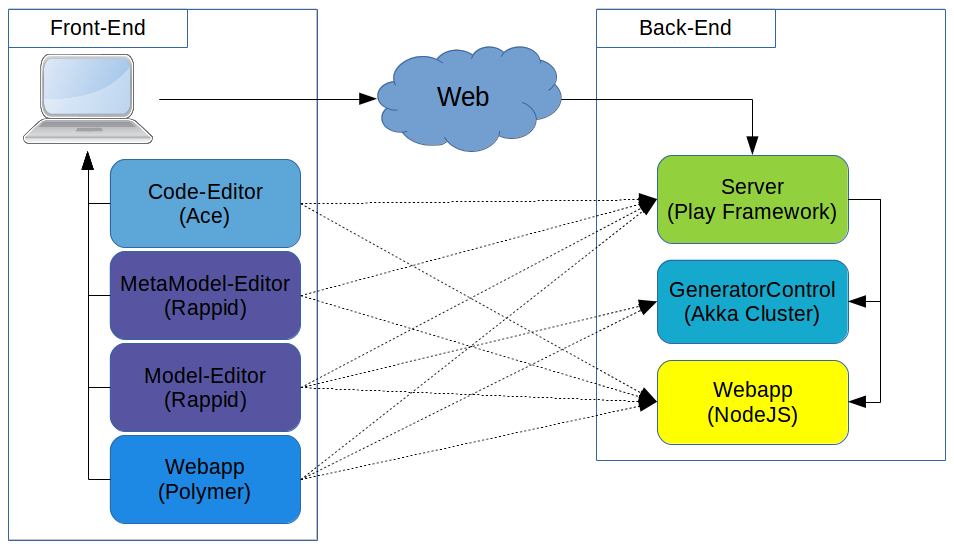
\includegraphics[width=5in]{figures/overview-final.png}
    \caption{Zielzustand - Übersicht}
    \label{fig:ZETA_OVERVIEW_NEW}
\end{figure}

Der Code-Editor ist zur Bearbeitung der Definition über die textuellen \acp{dsl} Style, Shape und Diagram zuständig. Dabei baut der Code-Editor von \textit{Zeta} wie zuvor auf den webbasierten Code Editor \ac{ace} auf. Die Konfiguration und Initialisierung wurde zudem im Rahmen dieser Arbeit und in Zusammenarbeit mit Patrick Leber von \textit{ScalaJS} auf JavaScript portiert und die Hauptdatei ist \textit{webapp/src/code-editor.js} \cite{zeta_code_editor,zeta_commit_code_editor}. Aus diesem Grund ist die gesamte \textit{ScalaJS} Umgebung überflüssig geworden und im Scala Projekt konnten die Unterprojekte \textit{Client} und \textit{Shared} entfernt werden \cite{zeta_commit_remove_sbt_client,zeta_commit_remove_sbt_shared}. Eine direkte Nutzung des \ac{ace} Editor ist nicht möglich, da das JavaScript Module System von \ac{ace} nicht mit \textit{Webpack} kompatibel ist. Aus diesem Grund wird bei \textit{Zeta} der Umweg über die Browserify kompatible und somit auch \textit{Webpack} kompatible Variante namens \textit{brace} gegangen. Bei der Portierung zu JavaScript sind zudem erstmal die Kollaboration und Autospeichern Funktion des Code-Editors entfernt worden, da der gewählte Ansatz unter anderem auf der Datenbank eine erhöhte Last verursacht hat und eine zukünftige Lösung ohne Persistierung arbeiten soll.

Die graphischen Editoren umfassen den Concept- und den Model-Editor. Beide Editoren basieren auf dem properitären \textit{Rappid} Editor. Der ehemalige MetaModel-Editor wurde aufgrund einer Umbenennung der grundlegenden Datenstruktur zum Concept-Editor umbenannt. Die Konfiguration für den Concept-Editor ist statisch definiert und die ist im Rahmen dieser Arbeit vom \textit{Play Server} zu \textit{Webpack} migriert worden \cite{zeta_commit_resolve_via_webpack}. Eintrittspunkt für den Concept-Editor ist die \textit{webapp/src/graphical-meta-model-editor.js} Datei und von hier aus werden die für den Concept-Editor relevanten Dateien über das \ac{es6} Module System geladen. Der Model-Editor ist auch im Rahmen dieser Arbeit in weiten Teilen zu \textit{Webpack} migriert worden. Die Konfiguration ist aber anders als beim Concept-Editor spezifisch für jedes Projekt und muss deswegen dynamisch erzeugt werden. Aktuell basiert das Ganze noch darauf, dass die Definitionen der textuellen \acp{dsl} aus dem Code-Editor mit den Definitionen aus dem Concept-Editor über einen Parser namens \textit{SprayParser} in ein Model unter \textit{de.htwg.zeta.server.generator.model} überführt wird. Auf Basis dieses Models werden über Generatoren im \textit{Play Server} JavaScript-Dateien erzeugt und in der Datenbank persistiert. Beim Aufruf des Model-Editors im Browser werden diese JavaScript Dateien zur Konfiguration des \textit{Rappid} Editors neben der JavaScript Datei von \textit{Webpack} geladen. Langfristig soll dieser proprietäre Ansatz durch Daten aus der \ac{rest} \ac{api} ersetzt werden. Anhand der Daten aus der \ac{rest} \ac{api} wird im Browser dann die spezifische Konfiguration für den \textit{Rappid} Editor erzeugt. Im Rahmen dieser Arbeit und in Zusammenarbeit mit Jan Bodendorf wurde die Generierung der Konfiguration auf Basis der \ac{rest} \ac{api} implementiert, aber noch nicht in den Model-Editor eingebunden \cite{zeta_milestone_2}. Eine Dokumentation über das Schema der \ac{rest} \ac{api} für die Erzeugung der Konfiguration des Model-Editors existiert auch, aber die Implementierung wurde innerhalb des aktuellen Teamprojekts zeitlich nach hinter verlagert \cite{zeta_wiki_rest_api}.

Die Webapp ist eine \ac{spa} und basiert auf der \textit{Polymer} Bibliothek. Die Implementierung der Webapp befindet sich im Verzeichnis \textit{webapp/src/app/} und bietet die Oberfläche zur Verwaltung der Generatoren. Dies umfasst das Erstellen, Löschen und Ausführen von Generatoren. Des Weiteren können die Transformationsregeln für die Generatoren definiert werden. Zusätzlich können noch in Scala geschriebene Filter für das genutzte Meta Modell eines Generators definiert werden. Aufbauend auf den Generatoren können noch verschiedenartige Task wie z.B. ein \textit{Timed Task} definiert werden. Im Gegensatz zum Ausgangszustand ist die Webapp nicht mehr direkt an eine Datenbank angebunden, sondern nutzt zum Großteil eigens für die Webapp erstellte \ac{rest} \ac{api} Endpoints. Um dies zu ermöglichen wurde im Rahmen dieser Arbeit die Implementierung zur Interaktion mit dem Backend gänzlich ausgetauscht \cite{zeta_commit_webapp_persist}.

\section{Back-End}

Bei der Beschreibung des Backends wird auf eine die verschiedenen Teilbereiche und ihre Dienste eingegangen. Zunächst wird die auf Laufzeitumgebung per \textit{Docker Compose} eingegangen. Danach folgt die Aufteilung der primär in Scala geschriebenen Implementierung von \textit{Zeta} für das Back-End und der neu eingeführten Qualitätssicherung per statische Code Analyse und der Testabdeckung per Unittests. Als nächstes wird auf die Teilkomponenten des \textit{Play Server} eingegangen, wie den Webservices und Websocket \acp{api}. Abschließend wird \textit{Akka Cluster} zur Verwaltung der Generatoren und die Ausführung der Generatoren über eigene \textit{Docker Container} beschrieben.

\subsection{Docker Compose}

Die Laufzeitumgebung ist für \textit{Zeta} weiterhin per \textit{Docker Compose} definiert und ist im Vergleich zur Ausgangsarchitektur im Rahmen dieser Arbeit in wesentlichen Bereichen vereinfacht worden. Der \textit{Play Server} nimmt nun, wie in Abbildung~\ref{fig:ZETA_ARCH_NEW} auf Seite~\pageref{fig:ZETA_ARCH_NEW} zu sehen, sämtliche externen Anfragen stellvertretend für alle Dienst an und leitet diese gegebenenfalls an den \textit{GeneratorControl} oder den \textit{Webapp} Dienst weiter. Die meisten der Anfragen werden jedoch schon innerhalb des \textit{Play Servers} verarbeitet, da der \textit{Play Server} z.B. für sämtliche \ac{rest} \acp{api} zuständig ist. Für den \textit{Akka Cluster} wird nun minimal nur noch ein einziger Dienst benötigt. Dies wird durch die Trennung der Startparameter ermöglicht und somit kann jeweils der \textit{Master}, der \textit{Developer} oder der \textit{Worker} konfiguriert werden. Der \textit{GeneratorControl} benötigt weiterhin Zugriff auf die \textit{Docker} \ac{api} um die Generatoren über externe \textit{Docker Container} auszuführen. Die Generatoren benötigen weiterhin Zugriff auf die \textit{Mongodb} zur Persistierung und auf den \textit{Play Server} zum Starten von weiteren Generatoren. Inzwischen wird nur noch die eine MongoDB als zentrale Datenbank genutzt und der Zugriff ist nur innerhalb des Backend möglich.

\begin{figure}
    \centering
    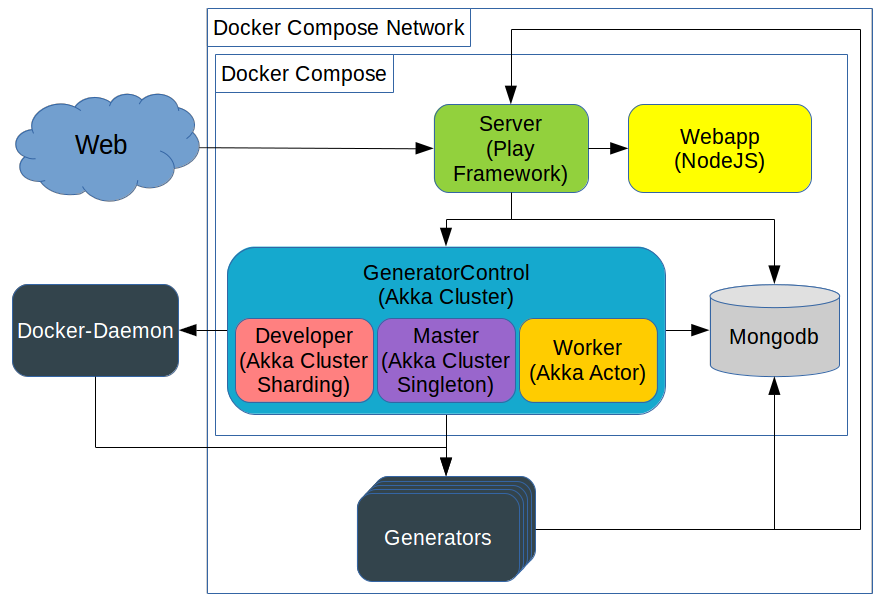
\includegraphics[width=5in]{figures/docker-compose-final.png}
    \caption{Zielzustand - Dienste}
    \label{fig:ZETA_ARCH_NEW}
\end{figure}

Zum Starten von \textit{Zeta} ist nun nur noch der Befehl \textit{docker-compose up} notwendig. Dies ist möglich indem nun für die Dienste nicht mehr über das Build Tool \ac{sbt} zuvor \textit{Docker Images} erzeugt werden müssen, sondern die Dienste wie der \textit{Play Server} und \textit{generatorControl} werden nun direkt über \ac{sbt} ausgeführt. Der Vorteil besteht darin, dass nun die verschiedensten \ac{sbt} Plugins für Entwicklersysteme genutzt werden können. Zuvor liefen die Dienste ohne \ac{sbt} und wurden direkt über gepackte JARs ausgeführt. Zum jetzigen Zeitpunkt wird aber kein offizielles \textit{Docker Image} für \ac{sbt} angeboten und die \textit{Docker Images} aus der Community sind entweder veraltet, bieten keine Auswahl einer spezifischen Java Version an oder haben nur eine Variante der offiziellen Java Images. Aus diesem Grund wurde ein eigenes \textit{Docker Image} für \ac{sbt} definiert und die genaue Definition kann im Programmcode~\ref{lst:ZETA_DOCKERFILE_SBT} auf Seite~\pageref{lst:ZETA_DOCKERFILE_SBT} nachvollzogen werden. Zuvor basierten die erzeugten \textit{Docker Images} für die Dienste auf \textit{openjdk:latest} mit einer unkomprimierten Gesamtgröße von 738 MB. Das eigene \textit{Docker Image} für \ac{sbt} basiert jedoch auf \textit{openjdk:8u151-jdk-alpine3.7} und ist mit einer unkomprimierten Gesamtgröße von 102 MB nur etwa 14\% der Größe des zuvor genutzten Images. Mit der Nutzung eines spezifischen \textit{Docker Image} ist nun auch die genutzte Java Version schon über den Namen des Image nachvollziehbar und die Kompatibilität zwischen den Entwicklersystem wird gewährleistet. Allgemein wurde nun bei allen Diensten auf die Nutzung eines spezifischen Images anstelle eines Bereichs verschiedener Versionen eines Images umgestellt.

\bigskip
\lstinputlisting[language=dockerfile, breaklines=true, caption={[SBT Dockerfile] SBT Dockerfile \cite{zeta_new_dockerfile}},label={lst:ZETA_DOCKERFILE_SBT}]{listings/Dockerfile.new}
\smallskip

Das \ac{sbt} Image wird nun wie im Programmcode~\ref{lst:ZETA_COMPOSE_GENERATOR} auf Seite~\pageref{lst:ZETA_COMPOSE_GENERATOR} genutzt um z.B. den \textit{generatorControl} Dienst zu definieren. Dabei ist zu sehen, dass das gesamte Scala Projekte aus dem Verzeichnis \textit{api} in den \textit{Docker Container} gemapped wird. Damit ist es nun möglich z.B. bei einen Neustart des Dienstes Änderungen zu kompilieren. Zusätzlich wird jeweils ein eigenes Verzeichnis für die \ac{sbt} Dateien wie dem Cache in das \textit{root} Verzeichnis gemapped. Des Weiteren werden die \textit{Docker} spezifischen Einstellungen nun über Umgebungsvariablen an den \textit{Docker Container} übergeben. Diese Erweiterung ist auch beim Dienst für den \textit{Play Server} durchgeführt worden. 

\bigskip
\lstinputlisting[language=docker-compose, breaklines=true, caption={[GeneratorControl Dienst - docker-compose.yml] GeneratorControl Dienst - docker-compose.yml \cite{zeta_new_docker_compose}},label={lst:ZETA_COMPOSE_GENERATOR}, firstline=3, lastline=14]{listings/docker-compose.new.yml}
\smallskip

Der \textit{webapp} Dienst basiert nun, wie in Programmcode~\ref{lst:ZETA_COMPOSE_WEBAPP} auf Seite~\pageref{lst:ZETA_COMPOSE_WEBAPP} zu sehen,  direkt auf dem offiziellen Image für \textit{Node.js} und nicht mehr wie zuvor auf einem eigens definierten Image \cite{zeta_webapp_image}. Ein Wechsel auf die minimale Alpine Variante ist nicht möglich gewesen, da dieser einige Abhängigkeiten wie z.B. die \textit{ace-grammer} Bibliothek nicht auf \ac{npm} zur Verfügung stehen und muss deshalb direkt von Github bezogen werden \cite{zeta_new_package_json}. Die Entscheidung zu Gunsten der um ein vielfaches größeren Standard Variante des \textit{Node.js} Image gegenüber eines eigenen Images mit Git auf Basis der Alpine Variante ist aufgrund der einfacheren Konfiguration des \textit{webapp} Dienstes gefallen. Ein eigens für die Webapp definiertes \textit{Docker Image} erhöht die Komplexität der \textit{Docker Compose} Konfiguration. Des Weiteren wird für den \textit{webapp} Dienst \textit{Yarn} als alternativer \ac{npm} Package Manager für eine schnellere Auflösung der Abhängigkeiten genutzt. Die Nutzung von \textit{Bower} als weiteren Package Manager ist nun direkt in den Installationsprozess der Abhängigkeiten von \textit{Yarn} integriert.

\bigskip
\lstinputlisting[language=docker-compose, breaklines=true, caption={[Webapp Dienst - docker-compose.yml] Webapp Dienst - docker-compose.yml \cite{zeta_new_docker_compose}},label={lst:ZETA_COMPOSE_WEBAPP}, firstline=42, lastline=47]{listings/docker-compose.new.yml}
\smallskip

Zur Laufzeit von \textit{Zeta} werden weiterhin mehrere \textit{Docker Images} zur Ausführung der Generatoren mit den Transformationsregeln benötigt. Diese Images können aber nun über den in \textit{Docker Compose} definierten \textit{images} Dienst erzeugt werden. Der Dienst kann per \textit{docker-compose up images} gestartet werden und beendet sich automatisch nach der Erzeugung der \textit{Docker Images}. Somit wird für den Betrieb von \textit{Zeta} nur noch \textit{Docker} mit \textit{Docker Compose} benötigt. Java oder auch \ac{sbt} muss auf dem Hostsystem nicht installiert werden, da dies über \textit{Docker Composer} abgefangen wird.  

\subsection{Scala Projekt}

Im Backend werden mehrere eigens für \textit{Zeta} entwickelte Dienste verwendet. Diese Dienste umfassen den \textit{Play Server}, den \textit{generatorControl} und die Generatoren. Dabei sind alle diese Dienste mit Scala implementiert und sind in einem gemeinsamen Scala Projekte im Verzeichnis \textit{api} zusammengefasst. Als Build Tool wird hierbei auf \ac{sbt} gesetzt. \textit{Zeta} nutzt einige Plugins für \ac{sbt} um z.B. eine Qualitätssicherung über Linter zu ermöglichen oder die verschiedenen Abhängigkeiten der Unterprojekte zu visualisieren. Eine Übersicht kann in der Tabelle~\ref{tab:ZETA_SBT_NEW} auf Seite~\pageref{tab:ZETA_SBT_NEW} gefunden werden. Im Gegensatz zur Ausgangsarchitektur aus dem Unterabschnitt~\ref{sec:INITIAL_BUILD} ab Seite~\pageref{sec:INITIAL_BUILD} wurden alle \ac{sbt} Plugins für \textit{SbtWeb} entfernt, da diese nicht länger benötigt werden.

\begin{table}[ht]
    \smallskip
    \centering
    \begin{tabular}{| l | l | l |}
    \hline
    \bf GroupID & \bf ArtifactID & \bf Beschreibung \\ \hline
    com.timushev.sbt & sbt-updates & Prüft auf neuere Versionen \\ \hline
    com.typesafe.play & sbt-plugin & Play Framework Dev Features \\ \hline
    com.typesafe.sbt & sbt-native-packager & Generiert Docker Images \\ \hline
    net.virtual-void & sbt-dependency-graph & Visualisiert Abhängigkeiten \\ \hline
    org.scalastyle & scalastyle-sbt-plugin & Scala Linter\\ \hline
    org.wartremover & sbt-wartremover & Scala Linter \\ \hline
    \end{tabular}
    \caption{Zielzustand - sbt Plugins \cite{zeta_new_sbt_plugins}}
    \label{tab:ZETA_SBT_NEW}
\end{table}

Die Implementierung innerhalb des \ac{sbt} Projekts ist in mehrere Unterprojekte aufgeteilt. Eine Übersicht der verschiedene Unterprojekte kann in Abbildung~\ref{fig:ZETA_SBT_NEW} auf Seite~\pageref{fig:ZETA_SBT_NEW} eingesehen werden. Dabei sind die genutzten Package Präfixe bei den verschiedenen Unterprojekten mit angegeben und enthalten untereinander keine zyklischen Abhängigkeiten. Der Umfang der verschiedenen Unterprojekte kann in der Tabelle~\ref{tab:ZETA_METRICS_LOC_NEW} auf Seite~\pageref{tab:ZETA_METRICS_LOC_NEW} eingesehen werden. Anders als z.B. ein Maven Projekt mit mehreren Modulen hat ein \ac{sbt} Projekt mit mehreren Unterprojekten nur eine gemeinsame Konfiguration für alle Unterprojekte. Von Nicolas Wehrle wurde jedoch die zentrale \textit{build.sbt} in eine \textit{built.sbt} pro Unterprojekt aufgeteilt.

Das \textit{Common} Projekt ist eines der zentralen Unterprojekte von dem alle anderen Unterprojekte abhängig sind und enthält unter anderem die Klassen für die Datenbank Entities. Aber auch einige hilfreiche Klassen für die \textit{Akka Actoren} und die Formatter für die Transformationen innerhalb der \ac{rest} \ac{api} und MongoDb Persistierung von \ac{json} zu einem Objekt und zurück. Auf dem \textit{Common} Unterprojekt baut wiederum mit dem \textit{Persistence} Projekt das zweite zentrale Unterprojekt auf. Das \textit{Persistence} Unterprojekt ist unter Patrick Leber neu zu \textit{Zeta} hinzugefügt worden und enthält die Implementierung für die Interaktion mit der MongoDB. Das umfasst die gängigen Aktionen wie z.B. Auslesen, Modifizieren, Löschen und Erstellen von Einträgen in der Datenbank. Die genutzte Implementierung für MongoDB wird über ein Module des \ac{di} Frameworks Guice konfiguriert und ersetzt die zuvor vorhandene Implementierung für Persistierung \cite{zeta_new_persistence_module}.

\begin{figure}
    \centering
    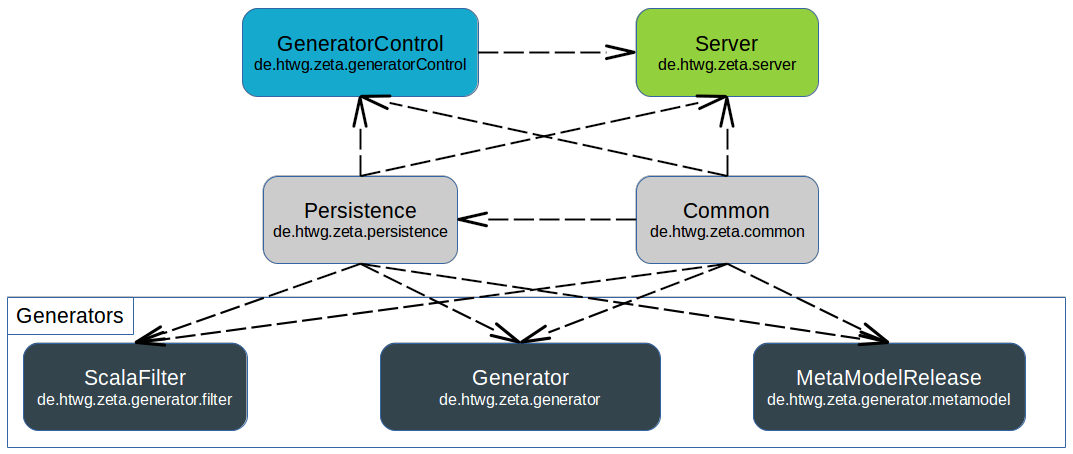
\includegraphics[width=5in]{figures/sbt-modules-final.png}
    \caption{Zielzustand - Abhängigkeiten der \ac{sbt} Unterprojekte}
    \label{fig:ZETA_SBT_NEW}
\end{figure}

\begin{table}[ht]
    \smallskip
    \centering
    \begin{tabular}{| l | r | r | r |}
    \hline
    \bf Projekt & \bf Gesamt & \bf SLOC & \bf CLOC \\ \hline
    common & 3937 (+570) & 2868 (+710) & 363 (-335) \\ \hline
    generatorControl & 2828 (+571) & 2183 (+471) & 167 (-28) \\ \hline
    scalaFilter & 144 (+19) & 119 (+105) & 3 (+3) \\ \hline
    generator & 528 (+528) & 377 (+377) & 92 (+92) \\ \hline
    metaModelRelease & 76 (+11) & 57 (+5) & 7 (+7) \\ \hline
    persistence & 3153 (+3153) & 2123 (+2123) & 520 (+520) \\ \hline
    server & 13657 (+3117) & 9650 (+2273) & 1731 (-107) \\ \hline
    \bf Gesamt & \bf 24323 (+5634) & \bf 17377 (+4118) & \bf 2883 (-83) \\ \hline
    \end{tabular}
    \caption{Zielzustand - \ac{loc} der Scala Dateien \cite{analys_new_directory}}
    \label{tab:ZETA_METRICS_LOC_NEW}
\end{table}

Der \textit{Play Server} befindet sich im \textit{Server} Unterprojekt und ist die öffentliche \ac{api} von \textit{Zeta}. Der \textit{Play Server} ist auf Basis des \textit{Play Frameworks} implementiert und hat nicht die Standard Maven Ordnerstruktur \cite{play_framework_anatomy}. Die Implementierung befindet sich im \textit{app} Verzeichnis, die Konfigurationsdateien wie z.B. die \textit{application.conf} oder \textit{routes} sind im \textit{conf} Verzeichnis und die Tests sind im \textit{test} Verzeichnis. Mit der Einführung von Package Präfixen unter Nicolas Wehrle sind die meisten Klassen des \textit{Play Server} in das Verzeichnis \textit{app/de/htwg/zeta/server} gewandert und entspricht somit nicht mehr der Standard Verzeichnisstruktur des \textit{Play Frameworks}. Der Aufbau des \textit{de.htwg.zeta.server} Paket kann in der Tabelle~\ref{tab:ZETA_NEW_PLAY_PACKAGES} auf Seite~\pageref{tab:ZETA_NEW_PLAY_PACKAGES} betrachtet werden. Im \text{app} Verzeichnis sind zusätzlich noch die Ordner \textit{controllers} mit der Konfiguration, ob eine Route nur für angemeldete Benutzer verfügbar ist, und das \textit{views} Verzeichnis mit den \ac{html} Templates. 

\begin{table}[ht]
    \smallskip
    \centering
    \begin{tabular}{| l | r | r | r | r | r |}
    \hline
    \bf Projekt & \bf Dateien & \bf Ordner & \bf Klassen & \bf Methoden & \bf Traits \\ \hline
    common & 65 (+29) & 13 (-3) & 167 (+0) & 194 (-33) & 28 (+12) \\ \hline
    generatorControl & 33 (+6) & 10 (+2) & 117 (+12) & 191 (+40) & 12 (-23) \\ \hline
    scalaFilter & 2 (+0) & 1 (-1) & 2 (+0) & 6 (+1) & 1 (+0) \\ \hline
    generator & 5 (+5) & 1 (+1) & 13 (+13) & 24 (+24) & 0 (+0) \\ \hline
    metaModelRelease & 1 (+0) & 1 (+0) & 2 (+0) & 0 (-1) & 0 (+0) \\ \hline
    persistence & 30 (+30) & 7 (+7) & 109 (+109) & 189 (+189) & 19 (+19) \\ \hline
    server & 232 (+78) & 49 (+2) & 407 (+138) & 1115 (+357) & 42 (+12)  \\ \hline
    \bf Gesamt & \bf 368 (+121) & \bf 82 (-3) & \bf 817 (+185) & \bf 1719 (+9) & \bf 102 (+6) \\ \hline
    \end{tabular}
    \caption{Zielzustand - Metriken über Scala Typen \cite{analys_new_directory}}
    \label{tab:ZETA_METRICS_NEW}
\end{table}

Das \textit{GeneratorControl} Unterprojekte basiert auf einem \textit{Akka Cluster} und ist für die Verwaltung der Generatoren zuständig \cite{akka_cluster}. Dabei werden die Anfragen von der Webapp aus dem Frontend verarbeitet und ein entsprechender Generator mit den Transformationsregeln über einen neuen \textit{Docker Container} ausgeführt. Die Generatoren umfassen die Unterprojekte \textit{ScalaFilter}, \textit{Generator} und \textit{MetaModelRelease}. Im Rahmen dieser Arbeit wurden die Unterprojekte \textit{BasicGenerator}, \textit{FileGenerator}, \textit{SpecificGenerator}, \textit{RemoteGenerator} und \textit{Template} aus der Abbildung~\ref{fig:ZETA_SBT_OLD} auf Seite~\pageref{fig:ZETA_SBT_OLD} zu dem Unterprojekte \textit{Generator} zusammengefasst. Diese Änderung wurde aufgrund der Bewertung der Generatoren aus dem Unterabschnitt~\ref{subsec:REVIEW_MODULES} ab Seite~\pageref{subsec:REVIEW_MODULES} durchgeführt und soll eine zu starke Modularisierung der Unterprojekte beheben.

\begin{table}[ht]
    \smallskip
    \centering
    \begin{tabular}{| l | l |}
    \hline
    \bf Paket & \bf Beschreibung \\ \hline
    actor & Akka Actoren \\ \hline
    controllers & Siehe \ac{mvc} Entwurfsmuster \\ \hline
    forms & Play Formular Definitionen \\ \hline
    generator & SprayParser und Models mit JavaScript Generatoren \\ \hline
    model & Meta Modell Actoren und Validator  \\ \hline
    module & Google Guice \ac{di} Module  \\ \hline
    routing & Mapper für Route auf Controller\\ \hline
    silhouette & Silhoutte Abhängige Authentifizierung \\ \hline
    start & Play Framework Bootstrap \\ \hline
    util & Allgemeine Hilfsklassen \\ \hline
    \end{tabular}
    \caption{Ausgangszustand - Play Server Pakete (de.htwg.zeta.server)}
    \label{tab:ZETA_NEW_PLAY_PACKAGES}
\end{table}

\subsection{Linter und Testabdeckung}

\textit{Zeta} verwendet in seinem Ausgangszustand nur die Linter des Scala Compilers zur längerfristigen Qualitätssicherung und die vorhandenen Unittests sind in einem nicht verwendbaren Zustand. Eine tiefere Beschreibung der Gesamtsituation kann im Unterabschnitt~\ref{subsec:REVIEW_QA} ab Seite~\pageref{subsec:REVIEW_QA} eingesehen werden. Wie in der Tabelle~\ref{tab:ZETA_SBT_NEW} auf Seite~\pageref{tab:ZETA_SBT_NEW} zusehen, verwendet \textit{Zeta} nun zusätzliche Linter. Die beiden Linter \textit{Wartremover} und \textit{Scalastyle} sind im Rahmen dieser Arbeit bei \textit{Zeta} ergänzt worden \cite{zeta_commit_linter,wartremover,scalastyle}. Der \textit{Wartremover} ist ein Plugin für den Scala Compiler und führt die Prüfungen beim Kompilieren der geänderten Scala Dateien aus. Die Konfiguration des \textit{Wartremover} für \textit{Zeta} meldet alle Probleme als Warnugen und bis auf den \textit{NonUnitStatements} sind alle Prüfungen aktiviert. \textit{Scalastyle} wiederrum kann z.B. über den \textit{scalastyle} Task per \ac{sbt} ausgeführt werden und ist zusätzlich an den \textit{Compile} Task von \ac{sbt} angehängt um ähnlich wie der \textit{Wartremover} beim Kompilierungsvorgang ausgeführt zu werden \cite{zeta_new_build}. Für \textit{Scalastyle} wird eine auf \textit{Zeta} angepasste Konfiguration verwendet und viele der gemeldeten Probleme wie z.B. vom \textit{UnderscoreImportChecker} sind im Rahmen dieser Arbeit behoben worden \cite{zeta_new_scalastyle,zeta_commit_UnderscoreImport}. Eine Übersicht der aktuell gemeldeten Probleme im Vergleich zum Ausgangszustand pro Unterprojekt befindet sich in der Tabelle~\ref{tab:ZETA_METRICS_LINT_NEW} auf Seite~\pageref{tab:ZETA_METRICS_LINT_NEW}.

\begin{table}[ht]
    \smallskip
    \centering
    \begin{tabular}{| l | r | r |}
    \hline
    \bf Projekt & \bf Compile with & \bf Scalastyle \\ 
    ~ & \bf Wartremover & (Err./War.) \\ 
    ~ & (Err./War.) & ~ \\ \hline
    common & 0 / 37 (0 / -50) & 0 / 82 (-67 / -151) \\ \hline
    generatorControl & 0 / 77 (+0 / -2) & 0 / 109 (-69 / -130) \\ \hline
    scalaFilter & 0 / 1 (+0 / -10) & 0 / 1 (-2 / -7) \\ \hline
    generator & 0 / 2 (+0 / +2) & 0 / 2 (+0 / +2) \\ \hline
    metaModelRelease & 0 / 0 (+0 / -2) & 0 / 0 (-1 / -4) \\ \hline
    persistence & 0 / 33 (+0 / +33) & 0 / 19 (+0 / +19) \\ \hline
    server & 0 / 563 (+0 / -267) & 0 / 922 (-264 / -1822) \\ \hline
    \bf Gesamt & \bf 0 / 713 (+0 / -411) & \bf 0 / 1135 (-437 / -2375) \\ \hline
    \end{tabular}
    \caption{Zielzustand - Ergebnisse der Linter Prüfungen \cite[Scalastyle]{analys_new}}
    \label{tab:ZETA_METRICS_LINT_NEW}
\end{table}

Für die Unittests wird einheitlich für alle Unterprojekt das Unittest Framework \textit{ScalaTest} verwendet und zur Prüfung der Testabdeckung wird zusätzlich \textit{scoverage} verwendet \cite{scalatest_project,scoverage}. Der aktuelle Stand der Unittests hat sich im Vergleich zum Ausgangszustand aus dem Unterabschnitt~\ref{subsec:REVIEW_QA} ab Seite~\pageref{subsec:REVIEW_QA} deutlich verändert. Der aktuelle Stand der Unittests und ihre Testabdeckung pro Unterprojekte befindet sich in der Tabelle~\ref{tab:ZETA_METRICS_TESTS_NEW} auf Seite~\pageref{tab:ZETA_METRICS_TESTS_NEW}. Sind im Ausgangszustand nur ingesamt drei Unittests vorhanden gewesenen, sind es nun über 800 verschiedene Unittests. Im Ausgangszustand konnte keiner der Unittests ausgeführt werden und nun können alle Unittests ausgeführt werden. Aktuell schlagen mit rund 3 \% aller Unittests einige der Unittests im \textit{Play Server} fehl. Die ermittelte Testabdeckung für Statements und Verzweigungen im Programmcode über alle Scala Dateien befindet sich nun im niedrigen zweistelligen Prozentbereich und ist im Vergleich zum Ausgangszustand ein ausreichender Zustand. Von einer minimalen Testabdeckung von z.B. 70 - 80 \% ist dies aber noch weit entfernt.

\begin{table}[ht]
    \smallskip
    \centering
    \begin{tabular}{| l | r | r | r | r |}
    \hline
    \bf Projekt & \bf Erfolgreich & \bf Fehlgeschlagen & \bf Statement & \bf Branch \\ \hline
    common & 1 & 0 & 5,57 \% & 0,00 \% \\ \hline
    generatorControl & 0 & 0 & 0,00 \% & 0,00 \% \\ \hline
    scalaFilter & 0 & 0 & 0,00 \% & 0,00 \% \\ \hline
    generator & 0 & 0 & 0,00 \% & 0,00 \% \\ \hline
    metaModelRelease & 0 & 0 & 0,00 \% & 0,00 \% \\ \hline
    persistence & 666 & 0 & 77,74 \% & 63,89 \% \\ \hline
    server & 134 & 21 & 10,03 \% & 16,54 \% \\ \hline
    \bf Gesamt & \bf 801 & \bf 21 & \bf 13,41 \% & \bf 16,24 \% \\ \hline
    \end{tabular}
    \caption{Zielzustand - Metriken über Unittests und Testabdeckung \cite[Scoverage]{analys_new_coverage,analys_new}}
    \label{tab:ZETA_METRICS_TESTS_NEW}
\end{table}

\subsection{Web \acp{api}}

Der \textit{Play Server} ist die öffentliche \ac{api} von \textit{Zeta} und stellt aus diesem Grund eine Reihe von Websockets und \ac{rest} Endpoints zur Verfügung. Eine Übersicht der verschiedenen Websockets kann in der Abbildung~\ref{fig:ZETA_WS_NEW} auf Seite~\pageref{fig:ZETA_WS_NEW} gefunden werden. Dabei ist der \textit{MetaModelWsActor} zusammen mit dem \textit{MetaModelWsMediatorActor} für den Abgleich zwischen mehreren Concept-Editor Instanzen für ein und dasselbe Projekt verantwortlich.

\begin{figure}
    \centering
    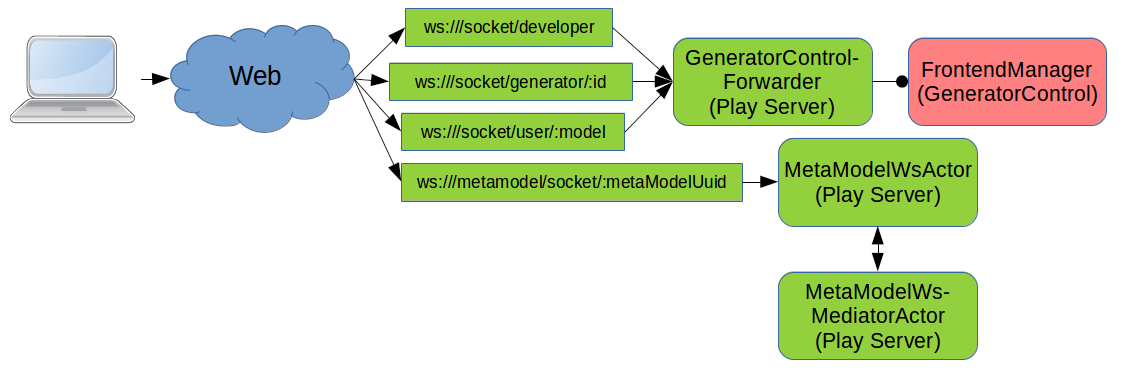
\includegraphics[width=5in]{figures/actor_play_final.png}
    \caption{Zielzustand - Websockets}
    \label{fig:ZETA_WS_NEW}
\end{figure}

Der \textit{Play Server} ist nun nicht mehr Teil des \textit{Akka Clusters} des {generatorControl} Dienst, sondern ist extern über einen Cluster Client an den \textit{generatorControl} Dienst angebunden. Die Anfragen von z.B. der Webapp werden über den \textit{GeneratorControlForwarder} Actor im \textit{Play Server} an den \textit{FrontendManager} Actor im \textit{generatorControl} Dienst \cite{akka_cluster_client} gesendet. Der \textit{FrontendManager} Actor gehört zur \textit{Developer} Node und sendet die Anfrage an den entsprechenden Actor innerhalb des \textit{Akka Clusters}.

\begin{table}[ht]
    \smallskip
    \centering
    \begin{tabular}{| l | l |}
    \hline
    \bf Method & \bf Route \\ \hline
    \colorbox{LimeGreen}{GET},\colorbox{LimeGreen}{POST} & /rest/v1/meta-models \\ \hline
    \colorbox{LimeGreen}{GET},\colorbox{red}{PUT} & /rest/v1/meta-models/:id \\ \hline
    \colorbox{LimeGreen}{DELETE} & /rest/v1/meta-models/:id \\ \hline
    \colorbox{red}{GET},\colorbox{LimeGreen}{PUT} & /rest/v1/meta-models/:id/definition \\ \hline
    \colorbox{red}{GET} & /rest/v1/meta-models/:id/definition/mclasses \\ \hline
    \colorbox{red}{GET} & /rest/v1/meta-models/:id/definition/mreferences \\ \hline
    \colorbox{red}{GET} & /rest/v1/meta-models/:id/definition/mclasses/:name \\ \hline
    \colorbox{red}{GET} & /rest/v1/meta-models/:id/definition/mreferences/:name \\ \hline
    \colorbox{red}{GET},\colorbox{LimeGreen}{PUT} & /rest/v1/meta-models/:id/shape \\ \hline
    \colorbox{red}{GET},\colorbox{LimeGreen}{PUT} & /rest/v1/meta-models/:id/style \\ \hline
    \colorbox{red}{GET},\colorbox{LimeGreen}{PUT} & /rest/v1/meta-models/:id/diagram \\ \hline
    \colorbox{LimeGreen}{GET} & /rest/v1/meta-models/:id/validator \\ \hline
    \colorbox{red}{PUT} & /rest/vl/meta-models/:id/classMethod/:method/:class \\ \hline
    \colorbox{red}{PUT} & /rest/vl/meta-models/:id/referenceMethod/:method/:ref \\ \hline
    \colorbox{red}{GET} & /rest/vl/meta-models/:id/commonMethod/:method \\ \hline
    \end{tabular}
    \caption{Zielzustand - Rest Endpoints MetaModel}
    \label{tab:ZETA_REST_META_NEW}
\end{table}

Auf Seiten der \ac{rest} \ac{api} Endpoints hat sich strukturell einiges verändert. Im Rahmen dieser Arbeit wurde der Prefix \textit{/rest/v1} zu allen \ac{rest} Endpoints hinzugefügt. Dies soll eine einfachere Unterscheidung zwischen einer Route zu einem \ac{html} Dokument und eines \ac{rest} Endpoints ermöglichen. Zusätzlich sollte durch das \textit{v1} eine Versionierung der \ac{rest} \ac{api} direkt erkennbar sein \cite{webservice_versioning}. Somit soll bei den Entwicklern für \textit{Zeta} ein stärkeres Bewusstsein für Breaking Changes hervorgerufen werden. Falls die Route eines \ac{rest} Endpoints geändert wird oder Umbenennungen im Schema stattfinden, kann dies zu Fehlern im Frontend führen. Eine Übersicht der \ac{rest} Endpoints für das Meta Modell und das Modell kann in der Tabelle~\ref{tab:ZETA_REST_META_NEW} auf Seite~\pageref{tab:ZETA_REST_META_NEW} und in der Tabelle~\ref{tab:ZETA_REST_MODEL_NEW} auf Seite~\pageref{tab:ZETA_REST_MODEL_NEW} gefunden werden. In den Tabellen ist die Hintergrundfarbe bei der \ac{http} Methode ein Indikator für die Nutzung des Endpoints. Grün als Hintergrundfarbe bedeutet, dass der Endpoint innerhalb von \textit{Zeta} im Frontend genutzt wird. Rot als Hintergrundfarbe wiederum zeigt, dass der Endpoint nirgends in \textit{Zeta} genutzt wird. In den Tabellen sind viele ungenutzte \ac{rest} Endpoints für die \ac{http} \textit{GET} Methode zusehen, die in der Route \textit{/:id/definition} enthalten. Diese Routen werden immer spezifischer und dabei werden die Rückgaben aus dem Endpoint immer weiter gefiltert. Diese spezifischeren Endpoints bieten im Vergleich zu den allgemeineren \ac{rest} Endpoints aber nicht detailliertere Informationen an. Der aktuelle Ansatz nutzt die allgemeinen \ac{rest} Endpoints wie z.B. \textit{/rest/v1/meta-models/:id} und filtert die Rückgabe im Browser entsprechend der gegebenen Anforderungen.   

\begin{table}[ht]
    \smallskip
    \centering
    \begin{tabular}{| l | l |}
    \hline
    \bf Method & \bf Route \\ \hline
    \colorbox{red}{GET},\colorbox{LimeGreen}{POST} & /rest/v1/models \\ \hline
    \colorbox{red}{GET},\colorbox{red}{PUT},\colorbox{LimeGreen}{DELETE} & /rest/v1/models/:id \\ \hline
    \colorbox{red}{GET},\colorbox{LimeGreen}{PUT} & /rest/v1/models/:id/definition \\ \hline
    \colorbox{red}{GET} & /rest/v1/models/:id/definition/nodes \\ \hline
    \colorbox{red}{GET} & /rest/v1/models/:id/definition/nodes/:name \\ \hline
    \colorbox{red}{GET} & /rest/v1/models/:id/definition/edges \\ \hline
    \colorbox{red}{GET} & /rest/v1/models/:id/definition/edges/:name \\ \hline
    \colorbox{LimeGreen}{GET} & /rest/v1/models/:id/validation \\ \hline
    \end{tabular}
    \caption{Zielzustand - Rest Endpoints Model}
    \label{tab:ZETA_REST_MODEL_NEW}
\end{table}

Neben den \ac{rest} Endpoints für das Meta Modell und Modell sind durch die Entfernung des Zugriffs auf die Datenbank im Frontend der Webapp einige neue Endpoints hinzugekommen. Eine List der neuen \ac{rest} Endpoints befindet sich in der Tabelle~\ref{tab:ZETA_REST_APP_OLD} auf Seite~\pageref{tab:ZETA_REST_APP_OLD}. Die Hintergrundfarbe ist derselbe Indikator wie bei den beiden vorherigen Tabellen über die \ac{rest} Endoints für das Meta Modell und Modell. 

\begin{table}[ht]
    \smallskip
    \centering
    \begin{tabular}{| l | l |}
    \hline
    \bf Method & \bf Route \\ \hline
    \colorbox{LimeGreen}{GET} & /rest/v1/generator-images \\ \hline
    \colorbox{LimeGreen}{GET} & /rest/v1/generators \\ \hline
    \colorbox{red}{GET},\colorbox{LimeGreen}{DELETE} & /rest/v1/generators/:id \\ \hline
    \colorbox{LimeGreen}{GET},\colorbox{LimeGreen}{POST} & /rest/v1/filters \\ \hline
    \colorbox{red}{GET},\colorbox{LimeGreen}{DELETE} & /rest/v1/filters/:id \\ \hline
    \colorbox{LimeGreen}{GET} & /rest/v1/meta-model-releases \\ \hline
    \colorbox{LimeGreen}{GET},\colorbox{LimeGreen}{POST} & /rest/v1/bonded-tasks \\ \hline
    \colorbox{LimeGreen}{DELETE} & /rest/v1/bonded-tasks/:id  \\ \hline
    \colorbox{LimeGreen}{GET},\colorbox{LimeGreen}{POST} & /rest/v1/event-driven-tasks \\ \hline
    \colorbox{LimeGreen}{DELETE} & /rest/v1/event-driven-tasks/:id \\ \hline
    \colorbox{LimeGreen}{GET},\colorbox{LimeGreen}{POST} & /rest/v1/timed-tasks \\ \hline
    \colorbox{LimeGreen}{DELETE} & /rest/v1/timed-tasks/:id \\ \hline
    \colorbox{LimeGreen}{GET},\colorbox{LimeGreen}{PUT} & /rest/v1/files/:id/*name \\ \hline
    \end{tabular}
    \caption{Zielzustand - Rest Endpoints Webapp}
    \label{tab:ZETA_REST_APP_OLD}
\end{table}

\subsection{Generator Verwaltung}

Die Verwaltung der Generatoren findet innerhalb des \textit{generatorControl} Dienstes statt und basiert auf einem \textit{Akka Cluster}. Dabei besteht der \textit{Akka Cluster} aus den drei Cluster Nodes \textit{Developer}, \textit{Master} und \textit{Worker}. Eine Übersicht der Kommunikationswege der Actoren des Akka Clusters befindet sich in der Abbildung~\ref{fig:ZETA_ACTOR_NEW} auf Seite~\pageref{fig:ZETA_ACTOR_NEW} und eine Übersicht der Hierachie der verschiedenen Actoren ist in Abbildung~\ref{fig:ZETA_HIERACHY_NEW} auf Seite~\pageref{fig:ZETA_HIERACHY_NEW}. Anfragen des \textit{Play Servers} werden vom \textit{FrontendManager} Actor als Teil der \textit{Developer} Node angenommen. Dabei wird bei den Anfragen zwischen einem \textit{DeveloperRequest}, \textit{GeneratorRequest} oder \textit{UserRequest} unterschieden. Innerhalb des \textit{Developer} Node findet die Kommunikation direkt über Actor Referenzen statt \cite{akka_actor}. Die Anfragen werden als nächstes vom \textit{Mediator} Actor an einen der entsprechenden Manager Actor weitergeleitet. Diese Manager Actoren wandeln die Anfrage in einen \textit{Job} Nachricht um und senden diesen weiterhin innerhalb der \textit{Developer} Node an den \textit{WorkQueue} Actor.

\begin{figure}
    \centering
    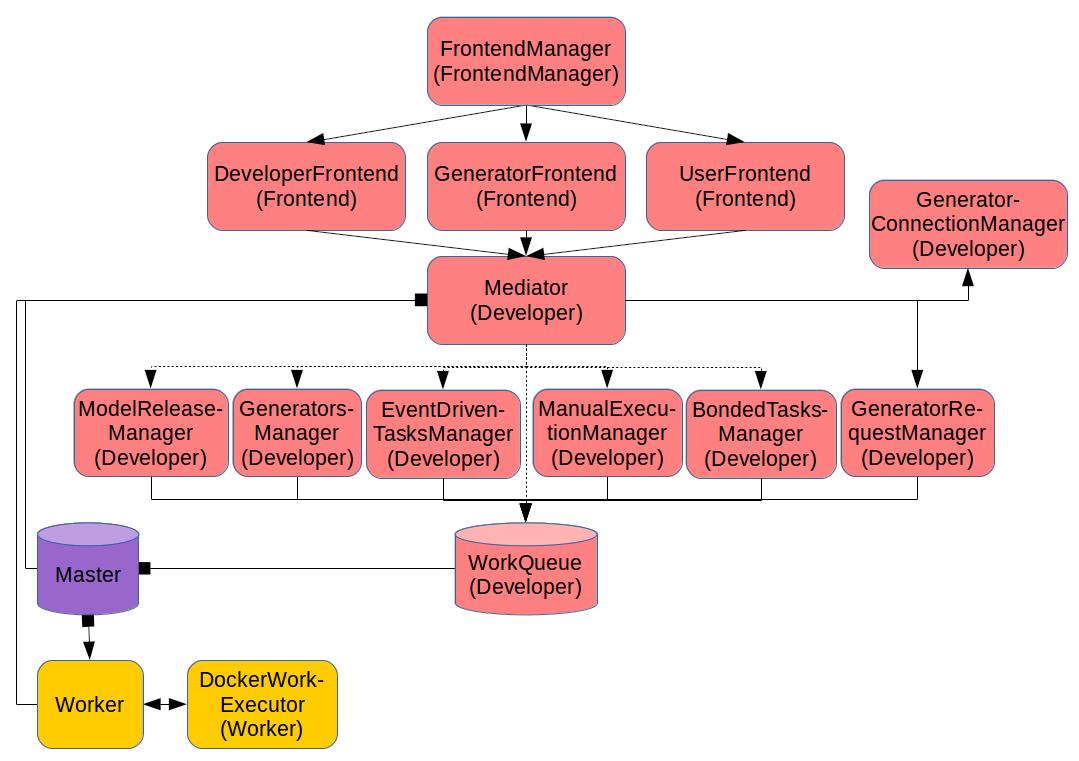
\includegraphics[width=5in]{figures/actor_backend_final.png}
    \caption{Zielzustand - Backend Actor System}
    \label{fig:ZETA_ACTOR_NEW}
\end{figure}

Der \textit{WorkQueue} Actor ist im Gegensatz zu den restlichen Actoren in der \textit{Developer} Node ein Persistent Actor mit einem internen Zustand der z.B. nach einem Absturz automatisch wiederhergestellt wird. Innerhalb des \textit{WorkQueue} Actor werden die \textit{Job} Nachrichten mit Zusatzinformation zu neuen Instanzen einer \textit{Work} Nachricht hinzugefügt und über den verteilten Publish Subscribe Mechanismus von Akka an den \textit{Master} Actoren der \textit{Master} Node gesendet \cite{akka_distributed_pub_sub}. Der \textit{Master} Node hat gegenüber der \textit{Developer} und \textit{Worker} Node die Sonderrolle als Seed Node innerhalb des \textit{Akka Clusters} und ist somit der Eintrittspunkt für alle Nodes, die dem \textit{Akka Cluster} beitreten wollen \cite{akka_cluster}. Der \textit{Master} Actor ist wie der \textit{WorkQueue} Actor ein Persistent Actor. Desweiteren enthält der \textit{Master} Actor eine interne List aller \textit{Worker} Actoren und den aktuellen Stand der abgearbeiteten \textit{Work} Objekte. Ein Rückkanal zur \textit{Developer} Node findet über den verteilten Publish Subscribe Mechanismus an den \textit{Mediator} Actor statt, der wiederrum die Nachricht an den \textit{WorkQueue} Actor weiterleitet.

Beim Empfang einer neuen \textit{Work} Nachricht im \textit{Master} Actor werden einige \textit{Worker} Actoren direkt per Actor Referenz über dieses Ereignis informiert. Die \textit{Worker} Actoren, die zu diesem Zeitpunkt Idle sind, versuchen diese neue \textit{Work} Nachricht zu übernehmen. Einer der \textit{Worker} Actoren bekommt dann vom \textit{Master} Actor den Zuschlag. Diese Koordination zwischen dem \textit{Master} und \textit{Worker} Actoren basiert auf einem Ansatz für verteilte Worker \cite{akka_worker_pull}. Ein Rückkanal zum \textit{Master} Actor der \textit{Master} Node und zum \textit{Mediator} Actor der \textit{Developer} Node findet wieder über den verteilten Publish Subscribe Mechanismus statt.

Der \textit{Worker} Actor überträgt das \textit{Work} Objekt an den eigenen \textit{DockerWorkExecutor} Actor über Actor Referenz innerhalb \textit{Worker} Node. Als nächstes übernimmt der \textit{DockerWorkExecutor} Actor die eigentliche Kommunikation mit dem \textit{Docker Daemon} zur Ausführung der \textit{Docker Container} für die Generatoren mit den Transformationsregeln. Während der Laufzeit werden die Ausgaben des \textit{Docker Containers} über den \textit{Worker} Actor an den \textit{Mediator} Actor gesendet und der \textit{Mediator} Actor sendet die Ausgaben wiederrum über den Websocket an den Browser. Wenn die Ausführung des \textit{Docker Containers} abgeschlossen ist, wird eine \textit{WorkComplete} Nachricht an den \textit{Worker} Actor gesendet. Der \textit{Worker} sendet wiederrum eine \textit{WorkIsDone} Nachricht an den \textit{Master} Actor. Der \textit{Master} Actor versendet schlussendlich eine \textit{MasterCompletedWork} Nachricht über den \textit{Mediator} Actor weitergeleitet an den \textit{WorkQueue} Actor zur Aktualisierung des internen Stands.

\begin{figure}
    \centering
    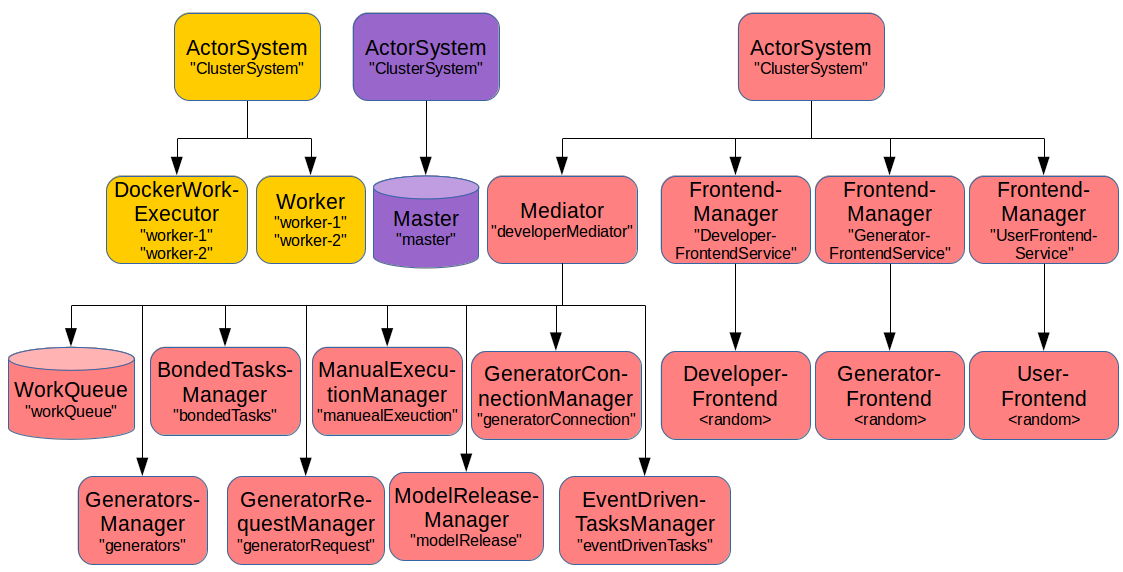
\includegraphics[width=5in]{figures/actor_hierachy_final.png}
    \caption{Zielzustand - Actor Hierachie}
    \label{fig:ZETA_HIERACHY_NEW}
\end{figure}

